\documentclass{sigchi}

% Use this command to override the default ACM copyright statement (e.g. for preprints). 
% Consult the conference website for the camera-ready copyright statement.


%% EXAMPLE BEGIN -- HOW TO OVERRIDE THE DEFAULT COPYRIGHT STRIP -- (July 22, 2013 - Paul Baumann)
% \toappear{Permission to make digital or hard copies of all or part of this work for personal or classroom use is 	granted without fee provided that copies are not made or distributed for profit or commercial advantage and that copies bear this notice and the full citation on the first page. Copyrights for components of this work owned by others than ACM must be honored. Abstracting with credit is permitted. To copy otherwise, or republish, to post on servers or to redistribute to lists, requires prior specific permission and/or a fee. Request permissions from permissions@acm.org. \\
% {\emph{CHI'14}}, April 26--May 1, 2014, Toronto, Canada. \\
% Copyright \copyright~2014 ACM ISBN/14/04...\$15.00. \\
% DOI string from ACM form confirmation}
%% EXAMPLE END -- HOW TO OVERRIDE THE DEFAULT COPYRIGHT STRIP -- (July 22, 2013 - Paul Baumann)


% Arabic page numbers for submission. 
% Remove this line to eliminate page numbers for the camera ready copy
\pagenumbering{arabic}


% Load basic packages
\usepackage{balance}  % to better equalize the last page
\usepackage{graphics} % for EPS, load graphicx instead
\usepackage{times}    % comment if you want LaTeX's default font
\usepackage{url}      % llt: nicely formatted URLs

% llt: Define a global style for URLs, rather that the default one
\makeatletter
\def\url@leostyle{%
  \@ifundefined{selectfont}{\def\UrlFont{\sf}}{\def\UrlFont{\small\bf\ttfamily}}}
\makeatother
\urlstyle{leo}


% To make various LaTeX processors do the right thing with page size.
\def\pprw{8.5in}
\def\pprh{11in}
\special{papersize=\pprw,\pprh}
\setlength{\paperwidth}{\pprw}
\setlength{\paperheight}{\pprh}
\setlength{\pdfpagewidth}{\pprw}
\setlength{\pdfpageheight}{\pprh}

% Make sure hyperref comes last of your loaded packages, 
% to give it a fighting chance of not being over-written, 
% since its job is to redefine many LaTeX commands.
\usepackage[pdftex]{hyperref}
\hypersetup{
pdftitle={SIGCHI Conference Proceedings Format},
pdfauthor={LaTeX},
pdfkeywords={SIGCHI, proceedings, archival format},
bookmarksnumbered,
pdfstartview={FitH},
colorlinks,
citecolor=black,
filecolor=black,
linkcolor=black,
urlcolor=black,
breaklinks=true,
}

% create a shortcut to typeset table headings
\newcommand\tabhead[1]{\small\textbf{#1}}


% End of preamble. Here it comes the document.
\begin{document}

\title{Glass Shooter: Exploring FPS Game Design with Google Glass}

\numberofauthors{3}
\author{
  \alignauthor Chun-Yen Hsu\\
    \affaddr{National Taiwan University}\\
    \affaddr{Mobile HCI Lab}\\
    \email{hcythomas0125@gmail.com}\\
  \alignauthor Ying-Chao Tung\\
    \affaddr{National Taiwan University}\\
    \affaddr{Mobile HCI Lab}\\
    \email{tony61507@gmail.com}\\
  \alignauthor Silvia Chyou\\
    \affaddr{National Taiwan University}\\
    \affaddr{Mobile HCI Lab}\\
    \email{silvia.chyou@gmail.com}\\
  \alignauthor Han-Yu Wang\\
    \affaddr{National Taiwan University}\\
    \affaddr{Mobile HCI Lab}\\
    \email{huw12313212@gmail.com}\\
  \alignauthor Wei-Jer Lin\\
    \affaddr{National Taiwan University}\\
    \affaddr{Mobile HCI Lab}\\
    \email{evin92@gmail.com}\\
  \alignauthor Mike Y. Chen\\
    \affaddr{National Taiwan University}\\
    \affaddr{Mobile HCI Lab}\\
    \email{belikemike@gmail.com}\\    
}

\maketitle

%\begin{figure}[!t]
%\centering
%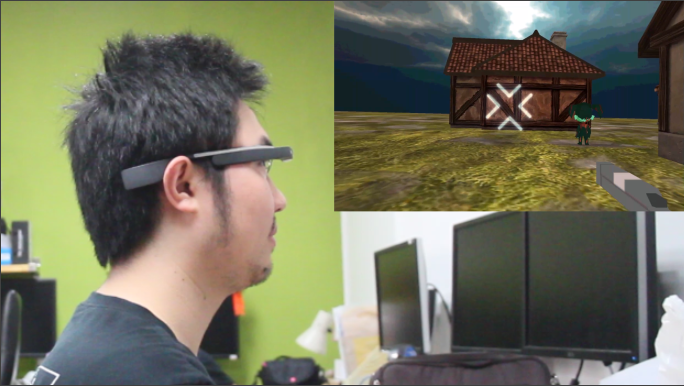
\includegraphics[width=0.9\columnwidth]{glassShooter.png}
%\caption{Glass Shooter gaming setting.}
%\label{fig:PS_Frus}
%\end{figure}


\begin{abstract}
Eyewear computers are claimed to be the next evolution beyond smartphones. In addition, game design for smart glass game is still an unexplored area. Hence, we want to explore the game design space on smart glass. For testing the current game play experience on google glass, we recruited 24 users to play four games on google glass with different content and control styles. By user feedback, about one third of users want to play First-Person Shooter(FPS) game. Hence, we implemented a FPS game on google glass and supply multiple control styles to evaluate and explore glass game design.
\end{abstract}

\keywords{
	Guides; instructions; author's kit; conference publications;
	keywords should be separated by a semi-colon.
	\textcolor{red}{Mandatory section to be included in your final version.}
}

\category{H.5.m.}{Information Interfaces and Presentation (e.g. HCI)}{Miscellaneous}

See: \url{http://www.acm.org/about/class/1998/}
for more information and the full list of ACM classifiers
and descriptors. 
\textcolor{red}{Mandatory section to be included in your
final version. On the submission page only the classifiers'
letter-number combination will need to be entered.}

\section{Introduction}
One of the most significant wearable computing break-throughs is Google's new ``eyewear computer'',expecting to be commercially available in 2014 referred to as Glass~\cite{glass}.
Eyewear computers are claimed to be the next evolution beyond smartphones. 

Game is one of the most important application in computer science. Recent statistics show that around 70~80\% of all mobile downloads is composed of mobile games\cite{statistics,infographic}. Traditional game design has tons of guidelines~\cite{videogame,mobilegame,bodygame,gameflow,argame,wearable}. However, it's lack of official research for smart glasses game design.

In our work, we want to explore the game design on smart glasses. We choose google glass, which has  several native glass games~\cite{minigame}, as our main research platform. To realize the current gameplay experience on google glass. We recruited 24 users to play 4 existing google glass game~\cite{minigame}, which has different game content and control style with each other. 

After analyzing users feedback, we found google glass has ``limited control'' issue. Compared to other gaming platform, there is no effective powerful input such as mouse, keyboard, joystick or touch screen. However, there are some non-traditional gaming input such as camera, small touch pad, microphone, gyroscope, and accelerometer. How to use these new control in glass game design is still an open question for people to discuss and explore. 

After user study, we found that about one third of users want to play First-Person Shooter(FPS) game on google glass. So we decide to implement a FPS game,``Glass Shooter'', on google glass for demonstration. In addition, we also provide multiple control styles to explore glass game design space and understand user preference.

%Eyewear computers, such as google glasses implementation, are claimed to be the next evolution beyond smartphones. In addition, game industry in the US earned about 21.53 dollars in 2014\cite{essentialfacts}. Recent statistics show that around 70-80\% of all mobile downloads is composed of mobile games\cite{statistics,infographic}. Traditional game design has tons of guidelines\cite{videogame,mobilegame,bodygame,gameflow,argame,wearable}. However, the game design for smart glass game is still an unexplored area. Hence, we want to explore the game design space on smart glass. And after concerning current market share, we choose Google Glass as our candidate.

%First we want to realize the current game play experience on google glass, so we recruited 24 users to play existing google glass game\cite{minigame} with different content or control style. After user study, we found that about one third of users want to play First-Person Shooter(FPS) game on google glass. So we decide to implement a FPS game on google glass for demonstration. In addition, we also provide multiple control styles to evaluate and find out the best control way on google glass. 

\section{Game Control Style}
In order to get deeper understanding of glass game design, we implement a game by ourself, which called ``Glass Shooter''. so that we can have some control variable to change directly by ourselves and compare with different settings. We also include smart phone as controller for our game designs and control scheme. We present 3 different control style, but they are not completely conflict with each other, player can just use them together or siwtch between each style. We described the control style below. 


\subsection{Glass Control}
First we just focus on google glass itself. In glass control, viewport is controlled by head orentation. By using the strip touchpad on the right side of google glass, player can move forward by pressing the front side of touchpad. By contrast, players also can move back by pressing the back side of touchpad. Scroll the touchpad can also change the viewport direction, to avoid big degree of head rotation. Player can use left tilt and right tilt to move left and right. And by tapping on touchpad, player can fire their weapon, such as gun or hand grenade. Finger slide

\subsection{Play with Controller}
We design to use smart phone as game controller. Reference to traditional gamepad controller, there are two joysticks on the phone, left one control player movement, right one rotate the viewport direction. Player can tap anywhere to fire the current weapon. In this case, player can still use head orientation to control viewport.

\subsection{Play with Metaphor}
To explore interaction between glass and phone, we also tried several experimental control with metaphor. Like hold your phone like a hand gun ,manipulate the phone orientation to aim the target and fire the gun by using index finger sliding the touch screen. Another metaphor is holding your phone as a hand grenade, player can use throw gesture to throw out the grenade. We also implement holding knife metaphor, player can brandish their phone to perform brandish knife attack.

%\subsubsection{Phone aiming}
% Aiming by using smart phone as a gun
%By using both of our hands, we can hold the smart phone with the same posture as we hold a gun. With this pose, we can switch our angle of view by revolving our body. And by using gyro, we can aim the target or the enemy by trimming our smart phone to shoot precisely. In other words, we can use smart phone as a aiming device, such as players using an electric torch or a gun.

%\subsubsection{Thrower}
% Using smart phone as body motion sensing
%Take Nintendo Wii for example, players movement can be detected precisely by the sensor. Although google glass can't have as strong sensor as Nintendo Wii, we still can detect some players' movement by our controller, smar phone. For instance, players hold the smart phone and can do throwing motion to simulate as throwing the hand grenade, and can make waving motion as waving the knife, and so on.

%\subsubsection{Driving simulation}
%While player driving the car, player use controller to emulate their motion as driving the car. It can indead raise players' game play experience greatly. So we can hold our controller, smart phone, as a steering wheel by both user's hand, and revolving the smart phone to emulate turning of the steering wheel.

%\subsubsection{Traditional joystick}
%To compare various of control method, we also provide traditional joystick for players on our controller, smart phone. By using traditional joystick, players can turning their angle of view and move their position directily.

\section{Conclusion}
In this demostration, we presented a first-person shooter game based on our user feedback from existing glass games. In order to explore the glass gaming control, which still an open question nowadays, so we designed and implemented multiple control styles; (a) Glass Control; (b) Play with Controller; (c) Play with Metaphor; We hope to inspire more glass game developer to develope more intuitive and suitable control. With better gaming control, we belive that it can enhance glass game play experience significantly than before, and we also hope to be able to inspire more exploration of smart glass gaming and spread game entertainment for more people.


\section{Acknowledgements}
We thank our advisor Prof. Mike Y. Chen and the faculty and staff of National Taiwan University. We should also like to express our gratitude towards all players and testers who have helped us in our many (buggy) iterations.

\balance

\bibliographystyle{acm-sigchi}
\bibliography{sample}
\end{document}
